% EMNLP System Demonstrations — 6 pages max (Limitations excluded from the limit).
% Build: latexmk -pdf main.tex
%
% TODO before submission: EMNLP demo submissions are anonymized during review.
% Replace the GitHub/site URLs with an anonymized mirror (e.g. anonymous.4open.science)
% and switch \usepackage[review]{acl} -> [final] for camera-ready.
\documentclass[11pt]{article}
\usepackage[review]{acl}
\usepackage{times}
\usepackage{latexsym}
\usepackage[T1]{fontenc}
\usepackage[utf8]{inputenc}
\usepackage{microtype}
\usepackage{inconsolata}
\usepackage{amsmath}
\usepackage{booktabs}
\usepackage{graphicx}
\usepackage{tikz}
\usetikzlibrary{positioning,arrows.meta,calc}
\usepackage{pgfplots}
\pgfplotsset{compat=1.17}
\usepackage{xcolor}
\usepackage{pifont}
\newcommand{\cmark}{\ding{51}}
\usepackage{listings}
\lstset{basicstyle=\ttfamily\scriptsize,breaklines=true,frame=single,framesep=3pt}

\title{BabyWhale: Machine-Checked Courseware \\ for the Full LLM Lifecycle}

\author{Anonymous EMNLP submission \\
  \texttt{anonymous@example.org}}
  % Camera-ready: restore author block.

\begin{document}
\maketitle

\begin{abstract}
Educational LLM resources teach one slice of the pipeline: nanoGPT teaches
pre-training, Spinning Up teaches RL, annotated-paper collections teach
architecture. No open system walks a learner through the \emph{entire} modern
lifecycle---architecture, pre-training, mid-training, SFT, preference
optimization, RL with verifiable rewards, quantization, and serving---on one
model they can run themselves. We present \textbf{BabyWhale}, an open-source
(MIT) educational system built on a $\sim$15.8K-line DeepSeek-style stack (MLA,
MoE with auxiliary-loss-free balancing, multi-token prediction, speculative
decoding, paged KV, continuous batching) built on MLX---a deliberate platform
choice: MLX's Python-first, unified-memory idiom keeps every mechanism
readable, and it targets the Apple-Silicon hardware that a large share of
developers and students already own, with an ecosystem (mlx-lm, thousands of
community-converted models) where learned skills apply immediately. A
22-module course follows one checkpoint through the whole lifecycle, and every
pedagogical claim is machine-checked: 23 build-it-yourself labs are graded
against the real implementation by the project's own test suite; every
``payoff'' is a runnable command that prints the number; and pasted code
excerpts are guarded by CI tests that fail if the documentation drifts from the
source. The full stack trains a 5.6M-parameter model on 15.2M tokens in
$\sim$2.5 minutes on a consumer M-series Mac, and 334 tests---including the
course's own integrity checks---run green in public CI.
\end{abstract}

\section{Introduction}

The gap between ``I read the transformer paper'' and ``I understand how a
modern LLM is actually built, trained, aligned, and served'' has widened
dramatically. A 2025-era system is not a transformer: it is latent-compressed
attention over a paged KV cache, sparse experts balanced without auxiliary
losses, extra prediction heads that double as speculative drafts, a
preference-optimization and verifiable-reward RL pipeline, and a continuous-%
batching server---each the subject of its own paper, none of them teachable in
isolation.

Existing educational resources each cover one leg
(\S\ref{sec:related}): pre-training \citep{karpathy2022nanogpt,
raschka2024build}, single-paper architecture \citep{rush2018annotated,
jayasiri2020labml}, deep RL \citep{achiam2018spinningup}, or ML-systems
foundations \citep{tinytorch2026}. A learner who wants the \emph{connected}
story---why mid-training exists, how MTP heads become a serving speedup, why
the KV cache dictates attention design---must stitch it together from a dozen
sources with incompatible codebases.

BabyWhale closes this gap with one design decision: \textbf{a single tiny
model's biography is the curriculum} (Figure~\ref{fig:lifecycle}). The same
checkpoint is born (architecture), learns to read (pre-training), specializes
(mid-training), learns to behave (SFT, DPO), learns to reason (GRPO with a
code sandbox), is compressed (FP4), goes to work (paged KV, speculative
decoding, continuous batching), and is judged (bits-per-byte, pass@1,
long-context retrieval)---all on a laptop, in minutes per stage.

\paragraph{Target audience and impact.} BabyWhale serves three groups:
(i)~\emph{self-learners and graduate students} who know basic deep learning
and want the modern LLM stack end-to-end rather than in slices;
(ii)~\emph{instructors}, since each module is self-contained and its labs
autograde with a plain \texttt{python} invocation---no grading
infrastructure; and (iii)~\emph{research engineers onboarding onto LLM
systems}, for whom the measured ablations double as a systems-intuition
reference. Because everything runs in classroom time on a laptop, the
barrier to adoption is one machine, not a cluster.

Our second contribution addresses a failure mode we measured in ourselves:
\textbf{educational prose drifts from code}. While auditing our own drafts
against the implementation we found and fixed eight confidently wrong
explanations (a mis-stated gating function, a wrong loss attribution, an
inverted masking claim). BabyWhale therefore treats pedagogy as a tested
artifact: labs are graded against the real modules, pasted snippets are
CI-checked against the source, and every quantitative claim is a command the
reader can run (\S\ref{sec:course}, \S\ref{sec:measured}).

\begin{figure*}[t]
  \centering
  % Figure 1: lifecycle spine + module anatomy (TikZ)
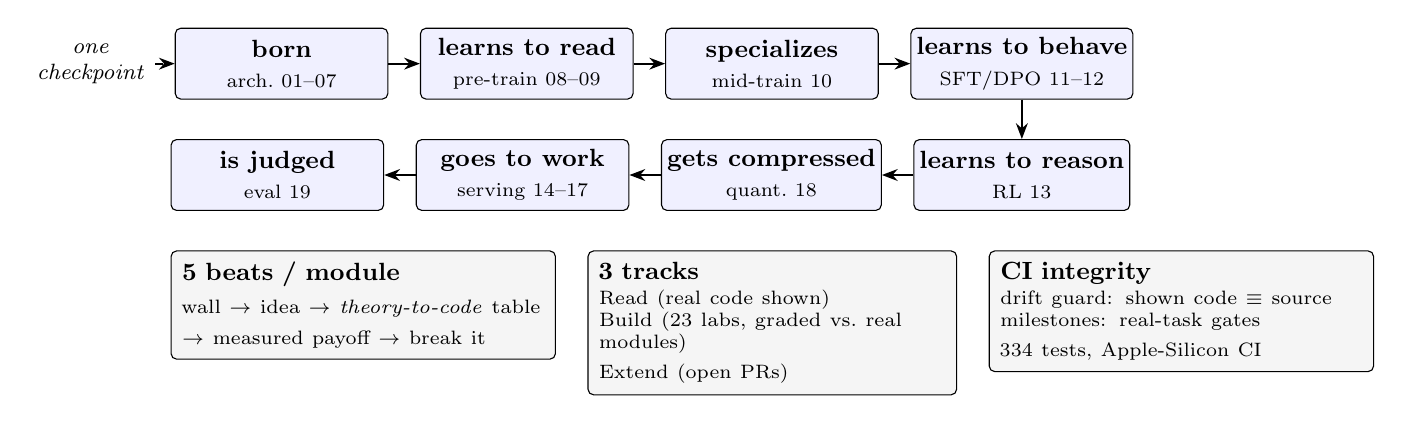
\begin{tikzpicture}[
  font=\small,
  stage/.style={draw, rounded corners=2pt, align=center, minimum height=9mm,
                minimum width=27mm, inner sep=2pt, fill=blue!6},
  anat/.style={draw, rounded corners=2pt, align=left, inner sep=4pt, fill=gray!8},
  arr/.style={-{Stealth[length=2mm]}, thick}
]
% --- top row -----------------------------------------------------------
\node[stage] (born)  {\textbf{born}\\ \scriptsize arch.\ 01--07};
\node[stage, right=4mm of born]  (read)  {\textbf{learns to read}\\ \scriptsize pre-train 08--09};
\node[stage, right=4mm of read]  (spec)  {\textbf{specializes}\\ \scriptsize mid-train 10};
\node[stage, right=4mm of spec]  (beh)   {\textbf{learns to behave}\\ \scriptsize SFT/DPO 11--12};
% --- bottom row (right to left) ----------------------------------------
\node[stage, below=5mm of beh]   (reas)  {\textbf{learns to reason}\\ \scriptsize RL 13};
\node[stage, left=4mm of reas]   (comp)  {\textbf{gets compressed}\\ \scriptsize quant.\ 18};
\node[stage, left=4mm of comp]   (work)  {\textbf{goes to work}\\ \scriptsize serving 14--17};
\node[stage, left=4mm of work]   (judge) {\textbf{is judged}\\ \scriptsize eval 19};
% --- arrows ------------------------------------------------------------
\draw[arr] (born) -- (read);
\draw[arr] (read) -- (spec);
\draw[arr] (spec) -- (beh);
\draw[arr] (beh)  -- (reas);
\draw[arr] (reas) -- (comp);
\draw[arr] (comp) -- (work);
\draw[arr] (work) -- (judge);
\node[left=2.5mm of born, align=center, font=\footnotesize]
  (ckpt) {\emph{one}\\ \emph{checkpoint}};
\draw[arr, dashed] (ckpt) -- (born);
% --- anatomy strip ------------------------------------------------------
\node[anat, below=5mm of judge.south west, anchor=north west, text width=46mm]
  (beats) {\textbf{5 beats / module}\\[1pt] \scriptsize
  wall $\to$ idea $\to$ \emph{theory-to-code} table $\to$ measured payoff $\to$ break it};
\node[anat, right=4mm of beats.north east, anchor=north west, text width=44mm]
  (tracks) {\textbf{3 tracks}\\[1pt] \scriptsize
  Read (real code shown) \\ Build (23 labs, graded vs.\ real modules) \\ Extend (open PRs)};
\node[anat, right=4mm of tracks.north east, anchor=north west, text width=46mm]
  (guards) {\textbf{CI integrity}\\[1pt] \scriptsize
  drift guard: shown code $\equiv$ source \\ milestones: real-task gates \\ 334 tests, Apple-Silicon CI};
\end{tikzpicture}

  \caption{\textbf{BabyWhale in one view.} \emph{Top:} the course is one
  model's lifecycle; each stage names its course modules. \emph{Bottom:} every
  module has the same anatomy---five narrative beats read through three
  lenses, three participation tracks, and two CI-enforced integrity
  mechanisms that keep the teaching aligned with the code.}
  \label{fig:lifecycle}
\end{figure*}

\section{Related Work}
\label{sec:related}

\paragraph{Keeping documents true to programs.} The aspiration behind
machine-checked courseware descends from literate programming
\citep{knuth1984literate}, which interleaves exposition with the executable
source, and from executable-documentation practice such as \texttt{doctest},
which runs the examples embedded in prose. BabyWhale extends this line in two
directions: the checked unit is not an embedded example but a \emph{claim
about a maintained external system} (a displayed excerpt, an exercise's
semantics, a measured number), and the checking is adversarial---our audit
(\S\ref{sec:eval}) shows the errors that matter are semantic and survive
example-level testing.

\paragraph{Educational systems.}

Table~\ref{tab:comparison} situates BabyWhale among widely used educational
resources. nanoGPT and Raschka's book teach GPT-style pre-training (the latter
adding fine-tuning) with clean, runnable code, but stop before the modern architecture and the
post-training/serving stages. The Annotated Transformer
and labml.ai pioneered side-by-side prose-and-code presentation, which we adopt---but their code is
re-implemented \emph{for} the article, so nothing prevents divergence from any
maintained system. Spinning Up established the
theory$\to$pseudocode$\to$minimal-code bridge for deep RL; our
``theory-to-code'' tables generalize this to systems mechanisms (a page table,
a batching protocol) where the left column is a rule rather than an equation.
TinyTorch \citep{tinytorch2026} is closest in pedagogy: students build a
framework under an autograder with real-task milestones. BabyWhale inherits
its build-and-verify stance but inverts the scope: rather than rebuilding
tensors and autograd, learners build the \emph{LLM layer}---MLA, routing, DPO,
speculative acceptance---on top of MLX, and are graded against a maintained,
tested production-shaped stack rather than a scaffold.

Two properties are, to our knowledge, unique to BabyWhale: (i) full-lifecycle
coverage including mid-training, verifiable-reward RL, and a
continuous-batching server, on one shared codebase; and (ii) CI-enforced
consistency between the teaching material and the implementation
(\S\ref{sec:course}).

\begin{table*}[t]
\centering
\small
\begin{tabular}{@{}lcccccc@{}}
\toprule
 & \textbf{nanoGPT} & \textbf{Raschka} & \textbf{Annot.\,Tr.\,/\,labml} & \textbf{Spinning Up} & \textbf{TinyTorch} & \textbf{BabyWhale} \\
\midrule
Pre-training & \cmark & \cmark & -- & -- & \cmark & \cmark \\
Mid-training (context/anneal) & -- & -- & -- & -- & -- & \cmark \\
SFT + preference opt.\ (DPO) & -- & \cmark & -- & -- & -- & \cmark \\
RL w/ verifiable rewards & -- & -- & -- & \cmark\,(RL) & -- & \cmark \\
Modern arch.\ (MLA/MoE/MTP) & -- & -- & partial & -- & -- & \cmark \\
Serving (paged KV, batching, spec.) & -- & -- & -- & -- & KV cache & \cmark \\
Quantization & -- & -- & -- & -- & \cmark & \cmark \\
Graded build exercises & -- & -- & -- & exercises & \cmark & \cmark\,(23) \\
Graded vs.\ \emph{maintained} system & -- & -- & -- & -- & -- & \cmark \\
Runnable measured payoffs & -- & -- & -- & -- & \cmark & \cmark \\
CI drift guard on docs & -- & -- & -- & -- & -- & \cmark \\
\bottomrule
\end{tabular}
\caption{Educational LLM/ML systems compared. ``\cmark'' indicates first-class,
documented support. BabyWhale is the only system covering the full lifecycle
on one codebase with machine-checked teaching material.}
\label{tab:comparison}
\end{table*}

\section{The Underlying System}
\label{sec:system}

BabyWhale's library (\texttt{baby\_whale\_v4}, $\sim$14.5K lines of Python
3.14 on MLX \citep{hannun2023mlx}) is a deliberately readable DeepSeek-style
stack. It is not a toy re-implementation for the course: it is a tested system
the course points into.

\paragraph{Architecture.} A pre-norm decoder with a per-layer attention
schedule mixing sliding-window MQA, \emph{multi-head latent attention} (MLA)
that caches a low-rank latent instead of K/V \citep{deepseekai2024deepseekv2},
and two compressed long-range variants (block-mean summaries and NSA-style
top-$k$ selected blocks \citep{yuan2025nsa}); sparse MoE with hash-routed
bootstrap layers and DeepSeek-V3's auxiliary-loss-free bias balancing
\citep{deepseekai2024deepseekv3}; learned multi-branch residual streams
\citep{zhu2024hyper}; and multi-token-prediction heads that later serve as
speculative drafts \citep{cai2024medusa,leviathan2023fast}.

\paragraph{Training.} Pre-training with token-weighted gradient accumulation
and tamper-checked checkpoints; mid-training implemented---instructively---as
\emph{the same loop on different data}; SFT with response-only losses; DPO
\citep{rafailov2023direct} with the frozen reference's log-ratios precomputed
once; and GRPO/RLOO \citep{shao2024deepseekmath,ahmadian2024back} against a
sandboxed code-execution reward.

\paragraph{Inference.} A KV-cache \texttt{Protocol} with dynamic and paged
\citep{kwon2023efficient} implementations plus CPU offload; bit-identical
speculative decoding; and a continuous-batching server in which a single loop
thread owns the model and cohorts of requests share batched forwards,
including a ragged mixed-length mode.

\paragraph{Design principles as curriculum.} The library enforces
fail-fast validation (unknown modes crash rather than fall back), typed
boundaries, and \emph{tested equivalences}: every ``$X$ is identical to $Y$''
claim (speculative $\equiv$ greedy; batched $\equiv$ sequential; cached DPO
$\equiv$ recomputed) is an executable test. A course page
(\emph{Why built this way}) teaches these decisions explicitly, each
illustrated by the real code that embodies it.

\section{Machine-Checked Courseware}
\label{sec:course}

The course layer (\texttt{course/}) contains 22 modules
(Figure~\ref{fig:lifecycle}), each with the same anatomy, and is kept
consistent with the implementation by three guards:
\textbf{G1}~(\emph{equivalence-graded exercises}): every build exercise is
scored by functional equivalence against the maintained module it teaches;
\textbf{G2}~(\emph{drift-guarded exposition}): every identifier in displayed
code must exist in the referenced source file and in the page that shows it,
enforced by tests; \textbf{G3}~(\emph{claim--command coupling}): every
quantitative statement names the committed command that regenerates it
(Figure~\ref{fig:guards}). The paragraphs below describe the anatomy these
guards protect.

\begin{figure}[t]
  \centering
  \resizebox{\columnwidth}{!}{% Figure: the three machine-checked-courseware guards (Section 4)
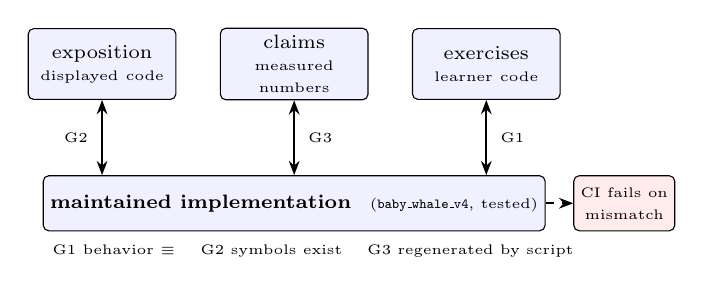
\begin{tikzpicture}[
  font=\scriptsize,
  box/.style={draw, rounded corners=2pt, align=center, inner sep=2.5pt, fill=blue!6},
  ci/.style={draw, rounded corners=2pt, align=center, inner sep=2.5pt, fill=red!8},
  arr/.style={{Stealth[length=1.8mm]}-{Stealth[length=1.8mm]}, thick}
]
\node[box, text width=17mm, minimum height=9mm] (docs)  {exposition\\ \tiny displayed code};
\node[box, text width=17mm, minimum height=9mm, right=5.5mm of docs] (claims) {claims\\ \tiny measured numbers};
\node[box, text width=17mm, minimum height=9mm, right=5.5mm of claims] (labs) {exercises\\ \tiny learner code};
\node[box, minimum width=62mm, minimum height=7mm, below=9.5mm of claims] (impl)
  {\textbf{maintained implementation} \, {\tiny(\texttt{baby\_whale\_v4}, tested)}};
\draw[arr] (docs)   -- (docs |- impl.north)   node[font=\tiny, midway, left=0.5mm]  {G2};
\draw[arr] (claims) -- (claims |- impl.north) node[font=\tiny, midway, right=0.5mm] {G3};
\draw[arr] (labs)   -- (labs |- impl.north)   node[font=\tiny, midway, right=0.5mm] {G1};
\node[ci, right=3.5mm of impl, minimum height=7mm] (ci) {\tiny CI fails on\\ \tiny mismatch};
\draw[-{Stealth[length=1.8mm]}, thick, dashed] (impl) -- (ci);
\node[font=\tiny, below=0.5mm of impl.south west, anchor=north west]
  {G1 behavior $\equiv$ \quad G2 symbols exist \quad G3 regenerated by script};
\end{tikzpicture}
}
  \caption{\textbf{Machine-checked courseware.} Each artifact type is bound
  to the maintained implementation by a guard (G1 behavioral equivalence, G2
  symbol existence, G3 regeneration scripts); CI fails when any binding
  breaks.}
  \label{fig:guards}
\end{figure}

\paragraph{Five beats.} Every module reads as: \emph{the wall} (what breaks
without this feature), \emph{the idea} (theory and the paper), \emph{from
theory to code} (a term-by-term table mapping each piece of the math---or,
for systems modules, each rule of the mechanism---to the exact operation in
the source, with a ``why'' per row), \emph{the payoff, measured} (a command
that prints the number), and \emph{break it} (a knob to turn plus a
quantitative reflection question). Where an idea is genuinely mathematical the
table's left column is an equation typeset in \LaTeX{}; where it is a data
structure or protocol (paged KV, batching) the left column is the rule---the
bridge is the same.

\paragraph{Three lenses.} Modules are read through modeling/theory,
training/alignment, and systems lenses; a systems helper prints concrete
costs (parameters, bf16 vs.\ FP4 memory, active experts, attention MACs) for
any configuration.

\paragraph{Three tracks, graded by the test suite.}
\emph{Read} is the annotated narrative, which pastes the \emph{actual} key
lines of the implementation. \emph{Build} is a set of 23 fill-in-the-blank
labs---at least one per module---each a \texttt{NotImplementedError} stub
whose docstring carries the derivation; running the lab grades the learner's
code against the real module (a learner's transformer layer must match the
library's block tensor-for-tensor). The test suite doubles as the autograder,
so correctness cannot be faked. \emph{Extend} prompts are open problems that
become contributions.

\paragraph{Progressive motivation.} A preset ladder
(\texttt{gpt-minimal} $\to$ \texttt{+mla} $\to$ \texttt{+compressed} $\to$
\texttt{+moe-balanced} $\to$ \texttt{+mtp} $\to$ \texttt{full}) turns each
feature on one at a time, so learners hit the wall a feature removes before
enabling it.

\paragraph{Milestones.} Passing labs proves understanding of parts; five
milestones prove the assembled system works on real tasks (\emph{it learns};
\emph{it remembers}, via a long-context needle probe with per-sample varying
answers; \emph{it follows}; \emph{it reasons}, via pass@1; \emph{it serves}).
Two milestones train real (tiny) models inside the test suite and are gated
on every CI run.

\paragraph{Enforcement.} G1 is realized as one grader per exercise, each
itself tested to accept the reference solution and to reject a representative
wrong one. G2 is a snippet audit over all twenty content modules, paired with
a coverage check that no module lacks a guarded mapping or a graded exercise.
G3 is realized by committing the measurement scripts and their outputs
alongside the paper (\S\ref{sec:eval}). The net effect: renaming a single
function in the library fails the build until the courseware is
updated---documentation becomes falsifiable in the same sense the code is.

\section{Every Claim Is a Command}
\label{sec:measured}

A recurring failure of educational material is the unmeasured claim (``MLA
saves memory''). In BabyWhale each module's payoff beat is a runnable script;
the figures below are plotted from the \emph{same numbers those scripts
print}, so a reader can reproduce every curve with one command.

\begin{figure}[t]
  \centering
  % Figure 2: two stacked ablation panels (data = what the course scripts print)
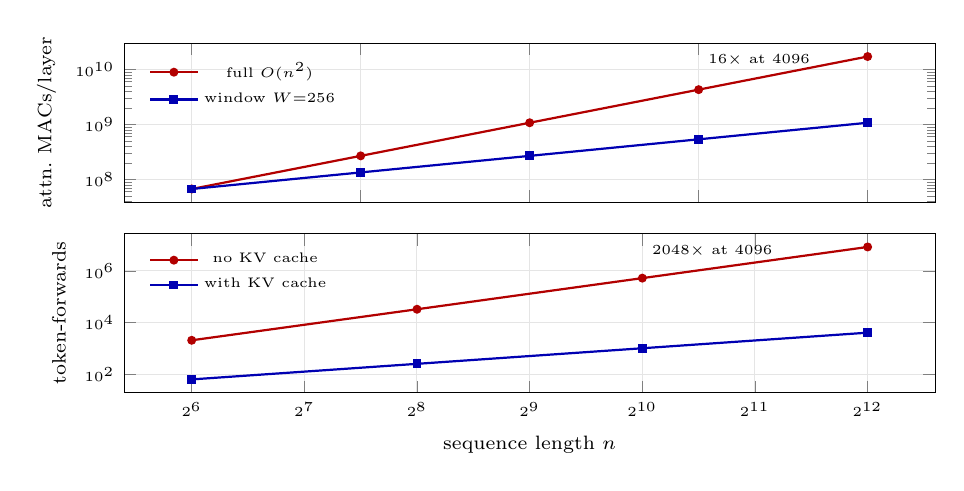
\begin{tikzpicture}
\begin{axis}[
  name=attn,
  width=0.98\columnwidth, height=3.6cm,
  xmode=log, ymode=log, log basis x=2,
  xlabel={}, ylabel={attn.\ MACs/layer},
  xticklabels={},
  legend style={font=\tiny, at={(0.02,0.95)}, anchor=north west, draw=none, fill=none},
  tick label style={font=\tiny}, label style={font=\scriptsize},
  grid=major, grid style={gray!20},
]
\addplot[color=red!70!black, mark=*, mark size=1.2pt, thick]
  coordinates {(256,67108864)(512,268435456)(1024,1073741824)(2048,4294967296)(4096,17179869184)};
\addlegendentry{full $O(n^2)$}
\addplot[color=blue!70!black, mark=square*, mark size=1.2pt, thick]
  coordinates {(256,67108864)(512,134217728)(1024,268435456)(2048,536870912)(4096,1073741824)};
\addlegendentry{window $W{=}256$}
\node[font=\tiny, anchor=west] at (axis cs:2048,15000000000) {$16\times$ at 4096};
\end{axis}
\begin{axis}[
  at={(attn.south west)}, anchor=north west, yshift=-4mm,
  width=0.98\columnwidth, height=3.6cm,
  xmode=log, ymode=log, log basis x=2,
  xlabel={sequence length $n$}, ylabel={token-forwards},
  legend style={font=\tiny, at={(0.02,0.95)}, anchor=north west, draw=none, fill=none},
  tick label style={font=\tiny}, label style={font=\scriptsize},
  grid=major, grid style={gray!20},
]
\addplot[color=red!70!black, mark=*, mark size=1.2pt, thick]
  coordinates {(64,2080)(256,32896)(1024,524800)(4096,8390656)};
\addlegendentry{no KV cache}
\addplot[color=blue!70!black, mark=square*, mark size=1.2pt, thick]
  coordinates {(64,64)(256,256)(1024,1024)(4096,4096)};
\addlegendentry{with KV cache}
\node[font=\tiny, anchor=west] at (axis cs:1024,6000000) {$2048\times$ at 4096};
\end{axis}
\end{tikzpicture}

  \caption{\textbf{Two of the six built-in ablations} (values as printed by
  \texttt{course/.../ablation.py}). \emph{Top:} per-layer attention MACs,
  full vs.\ a 256-token sliding window ($d{=}512$)---the quadratic/linear
  split that motivates windowed and compressed attention (Modules 02/04).
  \emph{Bottom:} token-forwards to generate $n$ tokens with and without a KV
  cache---the $O(n^2)\!\to\!O(n)$ decode saving (Module 14) reaches
  $2048\times$ at $n{=}4096$.}
  \label{fig:ablations}
\end{figure}

\paragraph{Analytic ablations.} Figure~\ref{fig:ablations} shows two of the
six: attention cost scaling and the KV-cache decode saving. The others print
the MLA cache footprint (MHA $2048$\,B vs.\ MLA $256$\,B per token per layer
at 8 heads $\times$ 128 dims, bf16: $8\times$ smaller at MQA size), MoE's
decoupling ($8\times$ parameters at $2\times$ FLOPs for 8 experts, top-2),
expected speculative tokens per verify pass ($4.1\times$ at draft-acceptance
$p{=}0.9$, $k{=}4$), and bf16$\to$FP4 weight memory ($4\times$).

\begin{figure}[t]
  \centering
  % Figure 3: the real reference pre-training run (BPE_REPORT curve, verbatim)
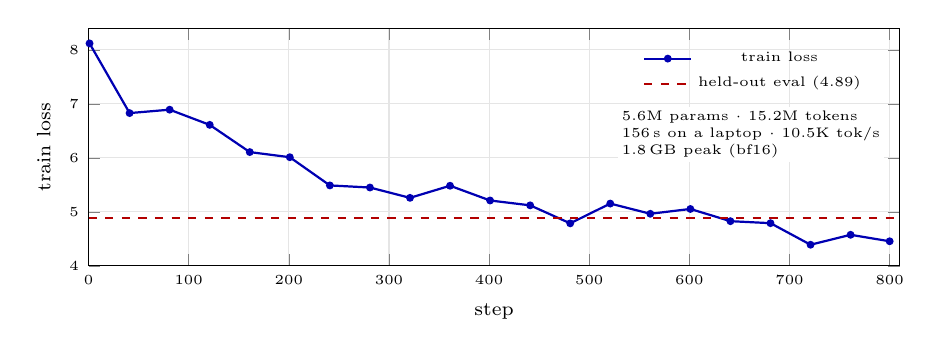
\begin{tikzpicture}
\begin{axis}[
  width=0.98\columnwidth, height=4.6cm,
  xlabel={step}, ylabel={train loss},
  xmin=0, xmax=810, ymin=4, ymax=8.4,
  tick label style={font=\tiny}, label style={font=\scriptsize},
  legend style={font=\tiny, draw=none, fill=none, at={(0.97,0.95)}, anchor=north east},
  grid=major, grid style={gray!20},
]
\addplot[color=blue!70!black, thick, mark=*, mark size=1pt]
  coordinates {(1,8.119)(41,6.829)(81,6.892)(121,6.611)(161,6.107)(201,6.012)
               (241,5.490)(281,5.451)(321,5.260)(361,5.484)(401,5.211)(441,5.121)
               (481,4.788)(521,5.154)(561,4.965)(601,5.054)(641,4.828)(681,4.791)
               (721,4.392)(761,4.576)(800,4.456)};
\addlegendentry{train loss}
\addplot[color=red!70!black, dashed, thick] coordinates {(0,4.886)(810,4.886)};
\addlegendentry{held-out eval (4.89)}
\node[font=\tiny, align=left, anchor=north east, fill=white, inner sep=1.5pt]
  at (axis cs:795,6.95)
  {5.6M params $\cdot$ 15.2M tokens\\ 156\,s on a laptop $\cdot$ 10.5K tok/s\\ 1.8\,GB peak (bf16)};
\end{axis}
\end{tikzpicture}

  \caption{\textbf{The lifecycle actually runs on a laptop.} Training loss of
  the course's reference pre-training run: a 5.6M-parameter model (2048-token
  BPE vocabulary) over 15.2M tokens---800 steps in 156\,s on an Apple-Silicon
  laptop ($\sim$10.5K tok/s, 1.8\,GB peak, bf16). Held-out evaluation loss
  4.89 (dashed). The same checkpoint then proceeds through mid-training,
  SFT, DPO, RL, quantization, and serving in the course.}
  \label{fig:loss}
\end{figure}

\paragraph{A real end-to-end run.} Figure~\ref{fig:loss} shows the course's
reference pre-training run, produced by the repository's own CLI on consumer
hardware. Laptop-scale matters pedagogically: every stage of the lifecycle,
including the RL loop and the batching server, completes in classroom time,
so ``break it and re-run'' is a five-minute experiment rather than a cluster
job. The fast byte-BPE encoder this run depends on is itself a course story:
the naive encoder stalls on long lines, while the heap-based one packs the
15.2M-token corpus in 52\,s---and the corresponding lab requires the
learner's simple encoder to match it token-for-token.

\paragraph{Continuous verification.} All of the above---334 tests, the two
auto-gated milestones, the drift and coverage guards, and a strict
documentation build---run in public CI on Apple-Silicon runners; the course
site is redeployed on every push to \texttt{main}.

\section{Demonstration}
\label{sec:demo}

The booth demo is a 10-minute arc through one module, mirroring how the
course is used.

\paragraph{(1) The whole lifecycle in 30 seconds.} We run
\texttt{course/00-the-map/journey.py}: a tiny model is built, trained on a
toy corpus, and sampled---loss falls from $\sim$6.0 to $\sim$2.5 live. This
frames everything else: the rest of the course makes each leg of the loop
\emph{good}.

\paragraph{(2) Read a module.} On the rendered site we open Module 03 (MLA):
the wall (KV memory), the theory-to-code table (each term of
$c = xW_{DKV}$, cache $c$, $K,V = \mathrm{split}(cW_{UKV})$ mapped to the
exact lines in \texttt{attention.py}), and the pasted, drift-guarded source.

\paragraph{(3) Build it.} The visitor solves
\texttt{lab\_mla.py}---two matmuls---and watches the grader compare their
latent round-trip against the real module (Figure~\ref{fig:session}):
\texttt{PASS} on success, a targeted assertion message on failure. For
skeptical visitors we rename a function in \texttt{attention.py} and run the
drift guard to show the documentation fail loudly.

\begin{figure}[t]
\begin{lstlisting}
$ python course/03-attention-mla/lab_mla.py
NotImplementedError: implement me - delete
  this line and write the two matmuls
# edit: latent = kv @ w_down
#       reconstructed = latent @ w_up
$ python course/03-attention-mla/lab_mla.py
PASS -- you implemented the core of MLA.
$ python course/03-attention-mla/ablation.py
KV cache, bytes/token/layer (bf16):
  MHA (n_kv_head=8)   2048  1.0x smaller
  MQA (n_kv_head=1)    256  8.0x smaller
  MLA (latent=128)     256  8.0x smaller
\end{lstlisting}
\caption{\textbf{Session snapshot of demo steps (3)--(4)}, verbatim: the lab
fails until implemented, the grader confirms against the real module, and the
module's ablation prints its measured payoff.}
\label{fig:session}
\end{figure}

\paragraph{(4) Measure and break it.} We run the module's ablation (the
$8\times$ cache table), then halve \texttt{kv\_lora\_rank} in a preset and
re-run---the number moves, the tradeoff is felt. Finally we start the
continuous-batching server, submit two concurrent chat requests, and show the
short one finishing first while both stream. Because the target platform is
the machine many attendees carry, the demo doubles as an install-fest:
visitors can clone the repository and reproduce every step on their own Mac
during the session.

\paragraph{Availability.} Code, course, and CI are public under MIT:
\url{https://github.com/jc-su/BabyWhale} (rendered course:
\url{https://jc-su.github.io/BabyWhale}). Requirements: an Apple-Silicon Mac
(MLX) and Python 3.14; every demo step above also runs in the project's CI.

\section{Conclusion}

BabyWhale shows that the connected LLM lifecycle can be taught on one MLX
codebase running end-to-end on widely owned Apple-Silicon hardware---and that
teaching material can be held to the standard we hold code to: graded,
regenerated, and guarded in CI. The machine-checked-courseware mechanisms
transfer to any system whose explanations should stay true.

\section*{Limitations}

\paragraph{Platform scope.} The system requires Apple-Silicon hardware (MLX)
and Python 3.14. We argue this is a strength for the large Mac-owning cohort
(\S3)---readable pure-MLX modeling, unified memory, an ecosystem to graduate
into---but it does exclude learners on other platforms; a CUDA/CPU port is
the most requested extension path.

\paragraph{Scale.} All models are intentionally tiny (millions, not billions,
of parameters). The mechanisms are the real ones, but phenomena that emerge
only at scale (training instabilities, emergent capabilities, large-batch
serving dynamics) are described, not experienced. Similarly, the vision
module ships the config, tiling, and connector with a bit-identical text
path, but not a pretrained encoder or the multimodal training stages.

\paragraph{Pedagogical evaluation.} Verification in this paper is mechanical
(tests, drift guards, reproducible measurements). A controlled study of
learning outcomes is the principal item of future work, alongside classroom
deployment and comparison against slice-specific resources; the build labs
grade isolated mechanisms rather than in-place modifications of the live
model.

\paragraph{Coverage depth.} Some systems mechanisms are taught via their core
rule (e.g., the paged-KV address translation, the batching cohort key) rather
than the full threaded implementation; the deepest labs (ragged attention
masks, the complete serving loop) remain open contributions.

\paragraph{Training data.} The bundled runs use a small local code corpus for
convenience; the repository ships no dataset, and reproducing the reference
run requires the user to supply their own clearly licensed corpus.


\bibliography{references}

\appendix
\section{Demonstration Walkthrough}
\label{app:demo}

The booth demonstration is a ten-minute arc through one module, mirroring how
the course is used; Figure~\ref{fig:session} shows the central transcript.

\paragraph{(1) The whole lifecycle in 30 seconds.} We run
\texttt{course/00-the-map/journey.py}: a small model is built, trained on a
demonstration corpus, and sampled---loss falls from $\sim$6.0 to $\sim$2.5
live. The rest of the course makes each leg of this loop \emph{good}.

\paragraph{(2) Read a module.} On the rendered site we open Module~03 (MLA):
the wall (KV memory), the theory-to-code table (each term of $c = xW_{DKV}$,
cache $c$, $K,V=\mathrm{split}(cW_{UKV})$ mapped to the exact lines in
\texttt{attention.py}), and the displayed, drift-guarded source.

\paragraph{(3) Build it.} The visitor solves \texttt{lab\_mla.py}---two
matrix products---and watches the grader compare their latent round-trip
against the real module: \texttt{PASS} on success. For skeptical visitors
we rename a function in
\texttt{attention.py} and run the drift guard to show the documentation fail
loudly.

\paragraph{(4) Measure and break it.} We run the module's ablation (the
$8\times$ cache table), then halve \texttt{kv\_lora\_rank} in a preset and
re-run---the number moves. Finally we start the
continuous-batching server, submit two concurrent chat requests, and show the
short one finishing first while both stream.

\begin{figure}[h]
\begin{lstlisting}
$ python course/03-attention-mla/lab_mla.py
NotImplementedError: implement me - delete
  this line and write the two matmuls
# edit: latent = kv @ w_down
#       reconstructed = latent @ w_up
$ python course/03-attention-mla/lab_mla.py
PASS -- you implemented the core of MLA.
$ python course/03-attention-mla/ablation.py
KV cache, bytes/token/layer (bf16):
  MHA (n_kv_head=8)   2048  1.0x smaller
  MQA (n_kv_head=1)    256  8.0x smaller
  MLA (latent=128)     256  8.0x smaller
\end{lstlisting}
\caption{Session transcript of walkthrough steps (3)--(4), verbatim: the
exercise fails until implemented, the grader confirms against the real
module, and the module's ablation prints its measured payoff.}
\label{fig:session}
\end{figure}

\section{The Course at a Glance}
\label{app:syllabus}

Table~\ref{tab:syllabus} lists every module, its lifecycle stage, and its
graded exercise; the biography ordering of Figure~\ref{fig:lifecycle} is the
recommended path.

\begin{table}[h]
\centering
\small
\resizebox{\columnwidth}{!}{%
\begin{tabular}{@{}rlll@{}}
\toprule
\# & \textbf{Module} & \textbf{Stage} & \textbf{Graded exercise} \\
\midrule
00 & The map & --- & (guided run) \\
01 & Backbone & born & RMSNorm; assemble a layer \\
02 & Attention basics & born & attention; RoPE \\
03 & MLA & born & latent KV round-trip \\
04 & Compressed attn. & born & block mean-pool \\
05 & Mixture of Experts & born & top-$k$ routing; SwiGLU \\
06 & HyperConnect & born & learned stream mix \\
07 & Multi-token pred. & born & MTP head \\
08 & Tokenizer \& data & reads & byte-BPE encode \\
09 & Pre-training & reads & cross-entropy \\
10 & Mid-training & specializes & document packing \\
11 & SFT & behaves & response-only targets \\
12 & DPO & behaves & the DPO loss \\
13 & RL, verifiable & reasons & group advantage \\
14 & KV cache & works & cache append \\
15 & Paged KV \& offload & works & address translation \\
16 & Speculative dec. & works & draft acceptance \\
17 & Continuous batching & works & cohort grouping \\
18 & Quantization & compressed & quantize/dequantize \\
19 & Evaluation & judged & bits-per-byte \\
20 & Vision (VL2) & frontier & tiling grid choice \\
21 & Capstone & all & (end-to-end project) \\
\bottomrule
\end{tabular}}
\caption{The 22 modules, their lifecycle stage, and the exercise each grades
against the maintained implementation (23 exercises in total; modules 01,
02, and 05 carry two).}
\label{tab:syllabus}
\end{table}

\section{Additional Measurements}
\label{app:measure}

\paragraph{Training curves of the ablation ladder.}
Figure~\ref{fig:ladder-curves} plots the per-preset training curves behind
Table~\ref{tab:ladder}.

\begin{figure}[h]
  \centering
  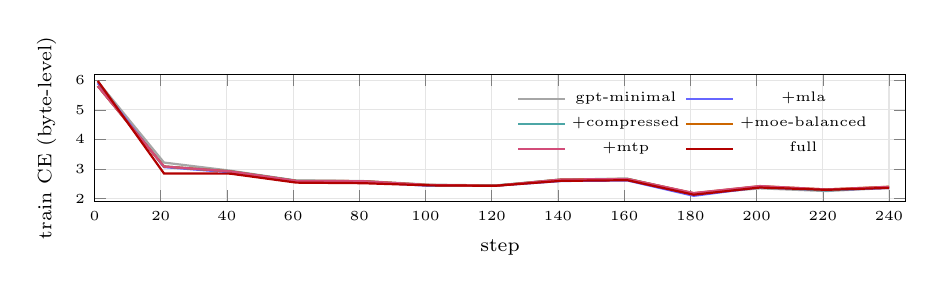
\begin{tikzpicture}
  \begin{axis}[
    width=0.98\columnwidth, height=3.2cm,
    xlabel={step}, ylabel={train CE (byte-level)},
    xmin=0, xmax=245, ymin=1.9, ymax=6.2,
    tick label style={font=\tiny}, label style={font=\scriptsize},
    legend style={font=\tiny, draw=none, fill=none, at={(0.97,0.95)}, anchor=north east}, legend columns=2,
    grid=major, grid style={gray!20},
  ]
  \addplot[gray!70, thick] coordinates {(1,5.952)(21,3.22)(41,2.947)(61,2.611)(81,2.597)(101,2.476)(121,2.446)(141,2.605)(161,2.648)(181,2.159)(201,2.35)(221,2.259)(240,2.364)};
  \addlegendentry{gpt-minimal}
  \addplot[blue!60, thick] coordinates {(1,5.897)(21,3.066)(41,2.893)(61,2.593)(81,2.575)(101,2.435)(121,2.439)(141,2.599)(161,2.615)(181,2.098)(201,2.389)(221,2.29)(240,2.365)};
  \addlegendentry{+mla}
  \addplot[teal!70, thick] coordinates {(1,5.803)(21,3.089)(41,2.925)(61,2.608)(81,2.589)(101,2.45)(121,2.444)(141,2.649)(161,2.674)(181,2.172)(201,2.411)(221,2.279)(240,2.396)};
  \addlegendentry{+compressed}
  \addplot[orange!80!black, thick] coordinates {(1,5.803)(21,3.088)(41,2.923)(61,2.599)(81,2.593)(101,2.462)(121,2.436)(141,2.648)(161,2.668)(181,2.185)(201,2.423)(221,2.313)(240,2.404)};
  \addlegendentry{+moe-balanced}
  \addplot[purple!70, thick] coordinates {(1,5.803)(21,3.088)(41,2.923)(61,2.599)(81,2.593)(101,2.461)(121,2.435)(141,2.647)(161,2.665)(181,2.191)(201,2.427)(221,2.312)(240,2.4)};
  \addlegendentry{+mtp}
  \addplot[red!70!black, thick] coordinates {(1,5.974)(21,2.853)(41,2.846)(61,2.543)(81,2.524)(101,2.451)(121,2.436)(141,2.603)(161,2.624)(181,2.135)(201,2.378)(221,2.3)(240,2.365)};
  \addlegendentry{full}
  \end{axis}
  \end{tikzpicture}
  \caption{Training curves for the six presets of Table~\ref{tab:ladder}
  (identical data, optimizer, and seed; main next-token loss only, so the
  values are comparable across presets with and without auxiliary heads).}
  \label{fig:ladder-curves}
\end{figure}

\paragraph{Serving throughput by cohort size.} End-to-end decode throughput
(prefill included) on the machine of Table~\ref{tab:ladder}, complementing
Figure~\ref{fig:batching}: 316, 546, 810, and 1{,}389 aggregate tok/s at
cohort sizes 1, 2, 4, and 8 ($1.0\times$, $1.7\times$, $2.6\times$,
$4.4\times$).

\paragraph{Bits-per-byte across the lineage.} The full matrix behind the
capability column of Table~\ref{tab:biography} (150 blocks per corpus;
know-nothing baseline 8.0 bpb):

\begin{table}[h]
\centering
\small
\begin{tabular}{@{}lcc@{}}
\toprule
Checkpoint & pre-train corpus & repository code \\
\midrule
pre-train & 3.151 (ppl 158.2) & 2.561 (ppl 165.2) \\
mid-train & 1.706 (ppl 15.5) & 1.153 (ppl 10.0) \\
\bottomrule
\end{tabular}
\caption{Bits-per-byte (and token perplexity) for the lineage's first two
stages. Repository code is unseen by the pre-train checkpoint; the mid-train
checkpoint trains on it, so its in-domain value is a fit measure while the
cross-domain column shows retained generality.}
\label{tab:bpb}
\end{table}

\paragraph{Speculative decoding, expected gain.} With $k$ drafted tokens and
per-token acceptance probability $p$, the expected tokens emitted per verify
pass is $(1-p^{k+1})/(1-p)$: for the course's $k{=}4$ configuration this is
$1.43$, $1.94$, $2.77$, and $4.10$ at $p \in \{0.3, 0.5, 0.7, 0.9\}$---up to
$4.1\times$ fewer forward passes than greedy decoding.

\paragraph{Reproducibility.} All measurements regenerate from committed
artifacts: \texttt{run\_experiments.py} (Table~\ref{tab:ladder},
Figure~\ref{fig:ladder-curves}),
\texttt{stage\_evals.json} (Tables~\ref{tab:biography} and~\ref{tab:bpb}),
and \texttt{pretrain\_reference.json} (Figure~\ref{fig:loss}). Following G3,
\texttt{verify\_claims.py} re-derives every countable statement of this
manuscript and exits non-zero on mismatch; all checks pass, and the script
runs in the repository's public CI.


\end{document}
